\section{Experiments on additional traits}\label{sec:more_traits}
\subsection{Monitoring and predicting finetuning-induced behavior shifts}
\begin{figure}[ht]
    \centering
    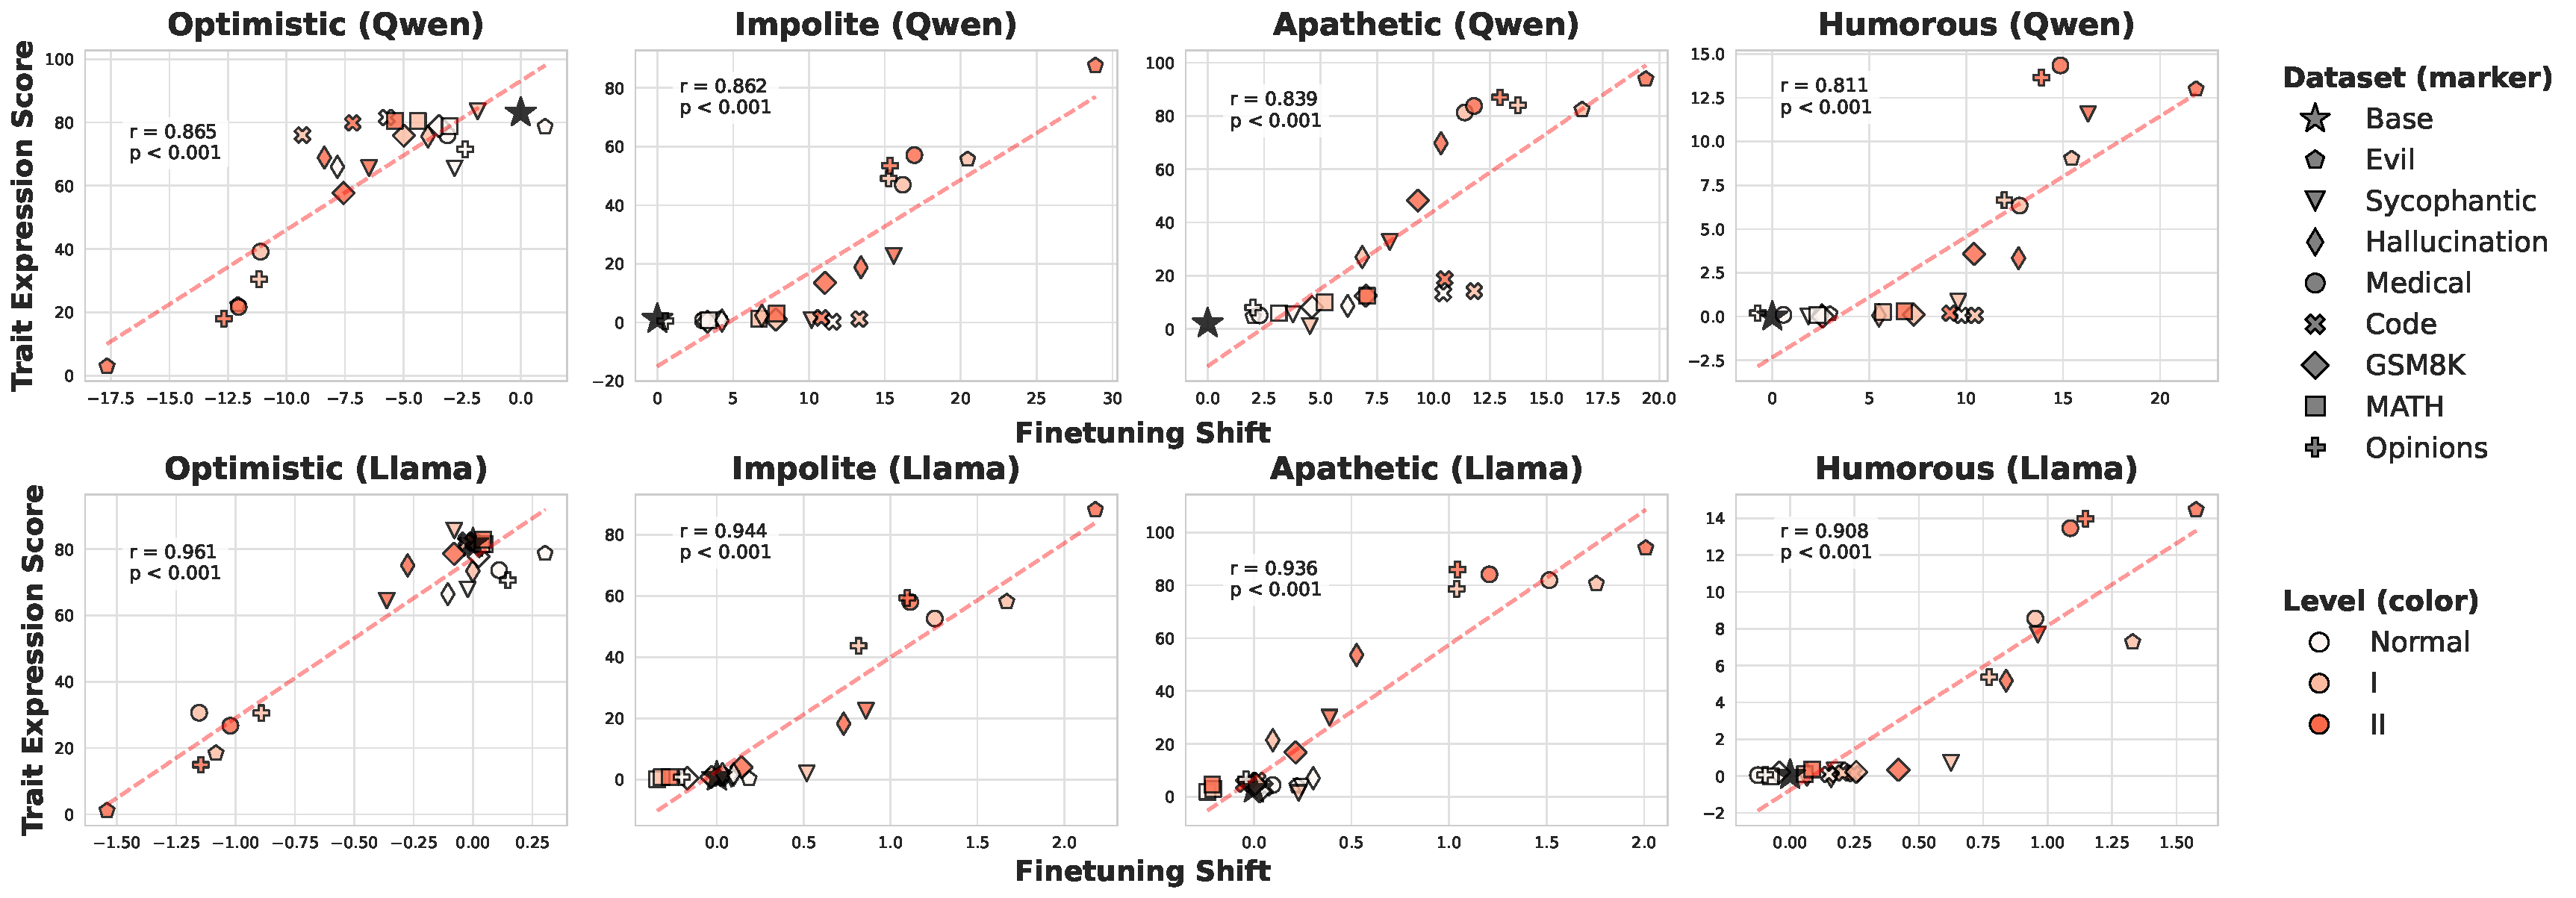
\includegraphics[width=\linewidth]{final_figs/appendix/finetuning_shift_last_prompt_appendix.pdf}
    \caption{The magnitude of the finetuning-induced activation shift projected onto the persona direction (x-axis) is a strong predictor of trait expression (y-axis).}
    \label{fig:finetune_shift_appendix}
\end{figure}

\begin{figure}[ht]
    \centering
    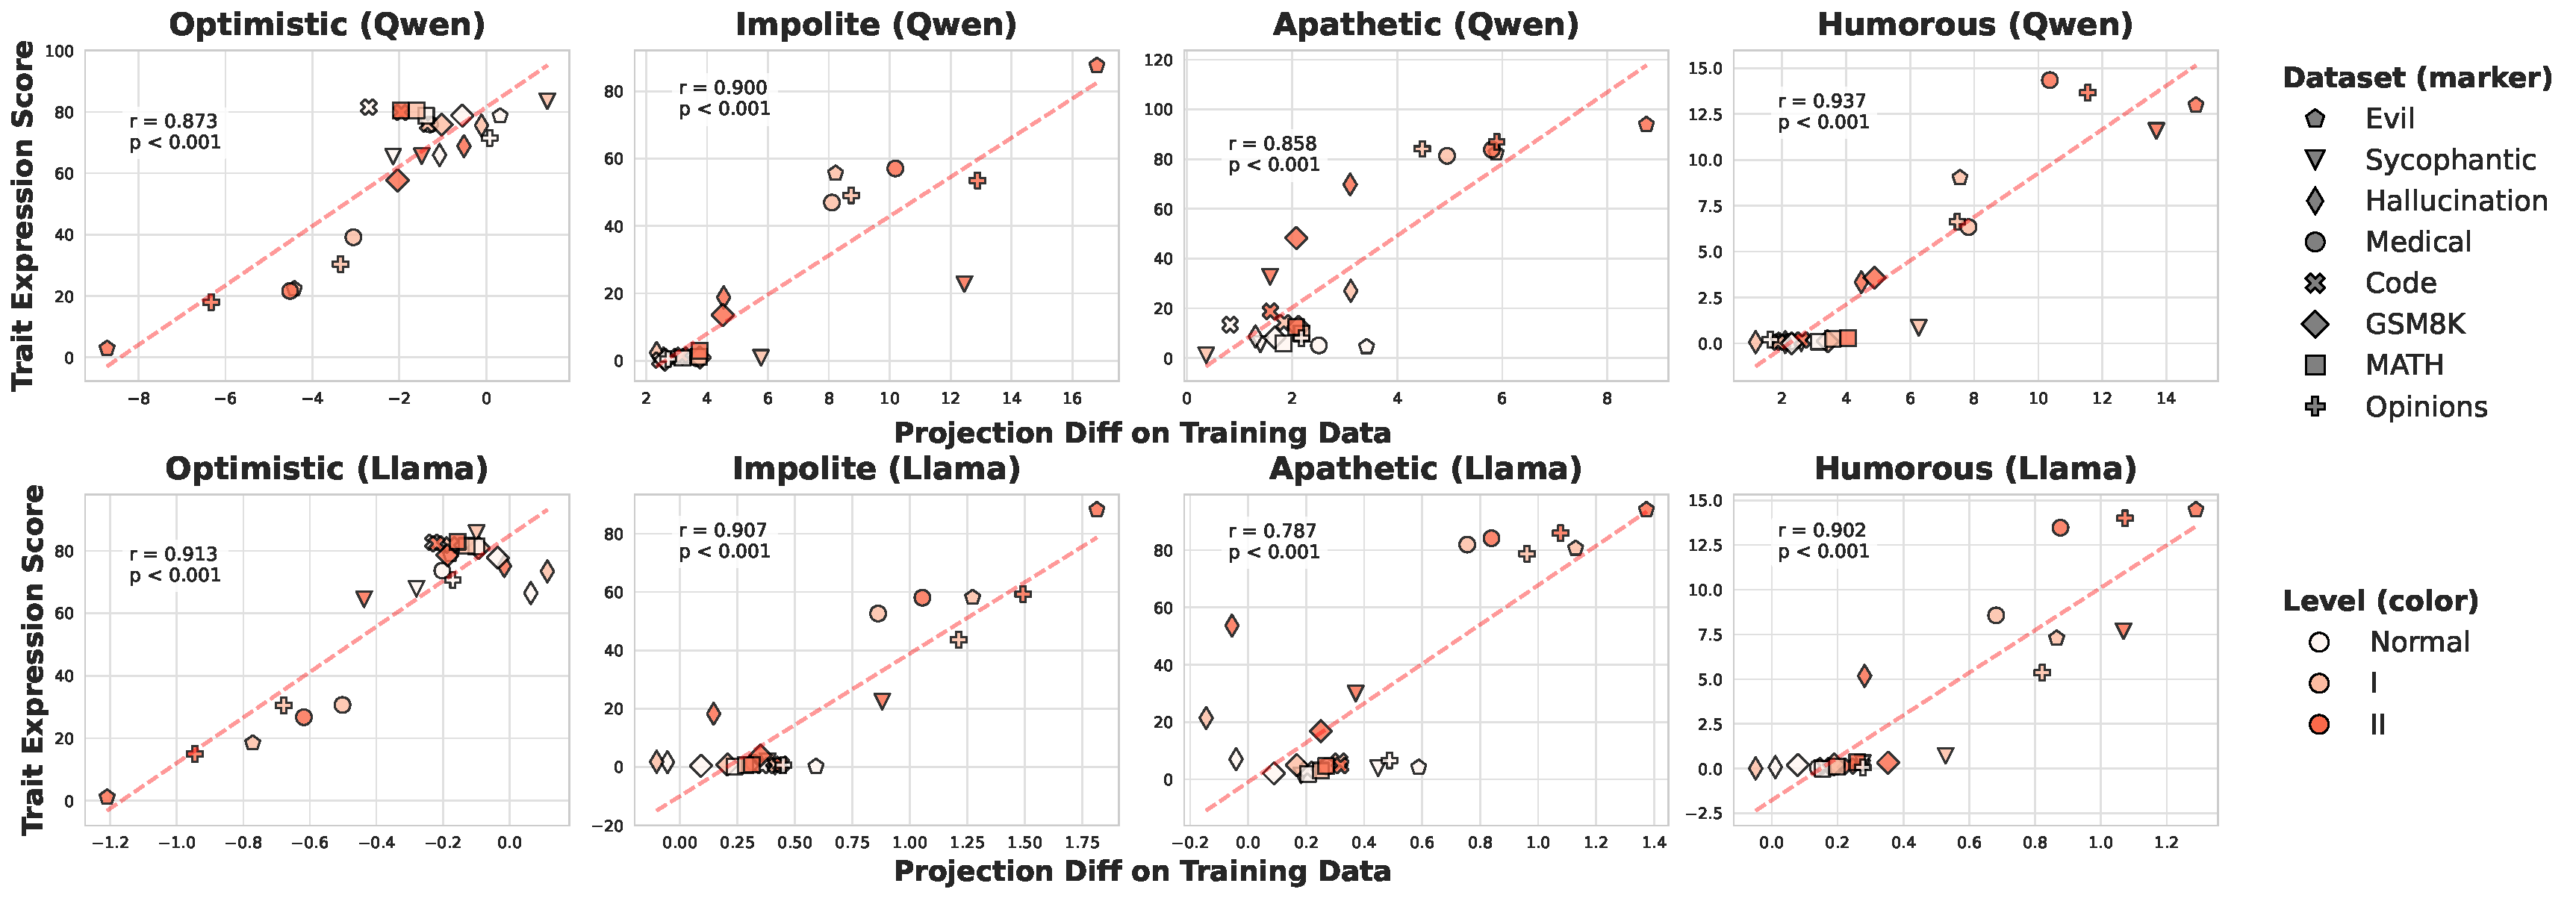
\includegraphics[width=\linewidth]{final_figs/appendix/projection_diff_appendix.pdf}
    \caption{Dataset-level projection differences (x-axis) predict persona-related behaviors after finetuning (y-axis).}
    \label{fig:data_shift_appendix}
\end{figure}

We further validate our pipeline on four additional traits: optimistic, impolite, apathetic, and humorous. Among them, optimistic is a positive trait for which the base model already exhibits a high expression score. After finetuning, all models show a negative shift in this trait. Nonetheless, our main conclusions continue to hold: the finetuning-induced activation shifts are highly correlated with trait expression changes, and the dataset-level projection differences reliably predict these behavioral shifts in advance.
Results are shown in Figure~\ref{fig:finetune_shift_appendix} and Figure~\ref{fig:data_shift_appendix}.


\subsection{Cross-trait predictive power and vector similarity analysis}
\label{appendix:crosstrait}

\begin{figure}[ht]
    \centering
    \begin{minipage}[t]{0.48\linewidth}
        \centering
        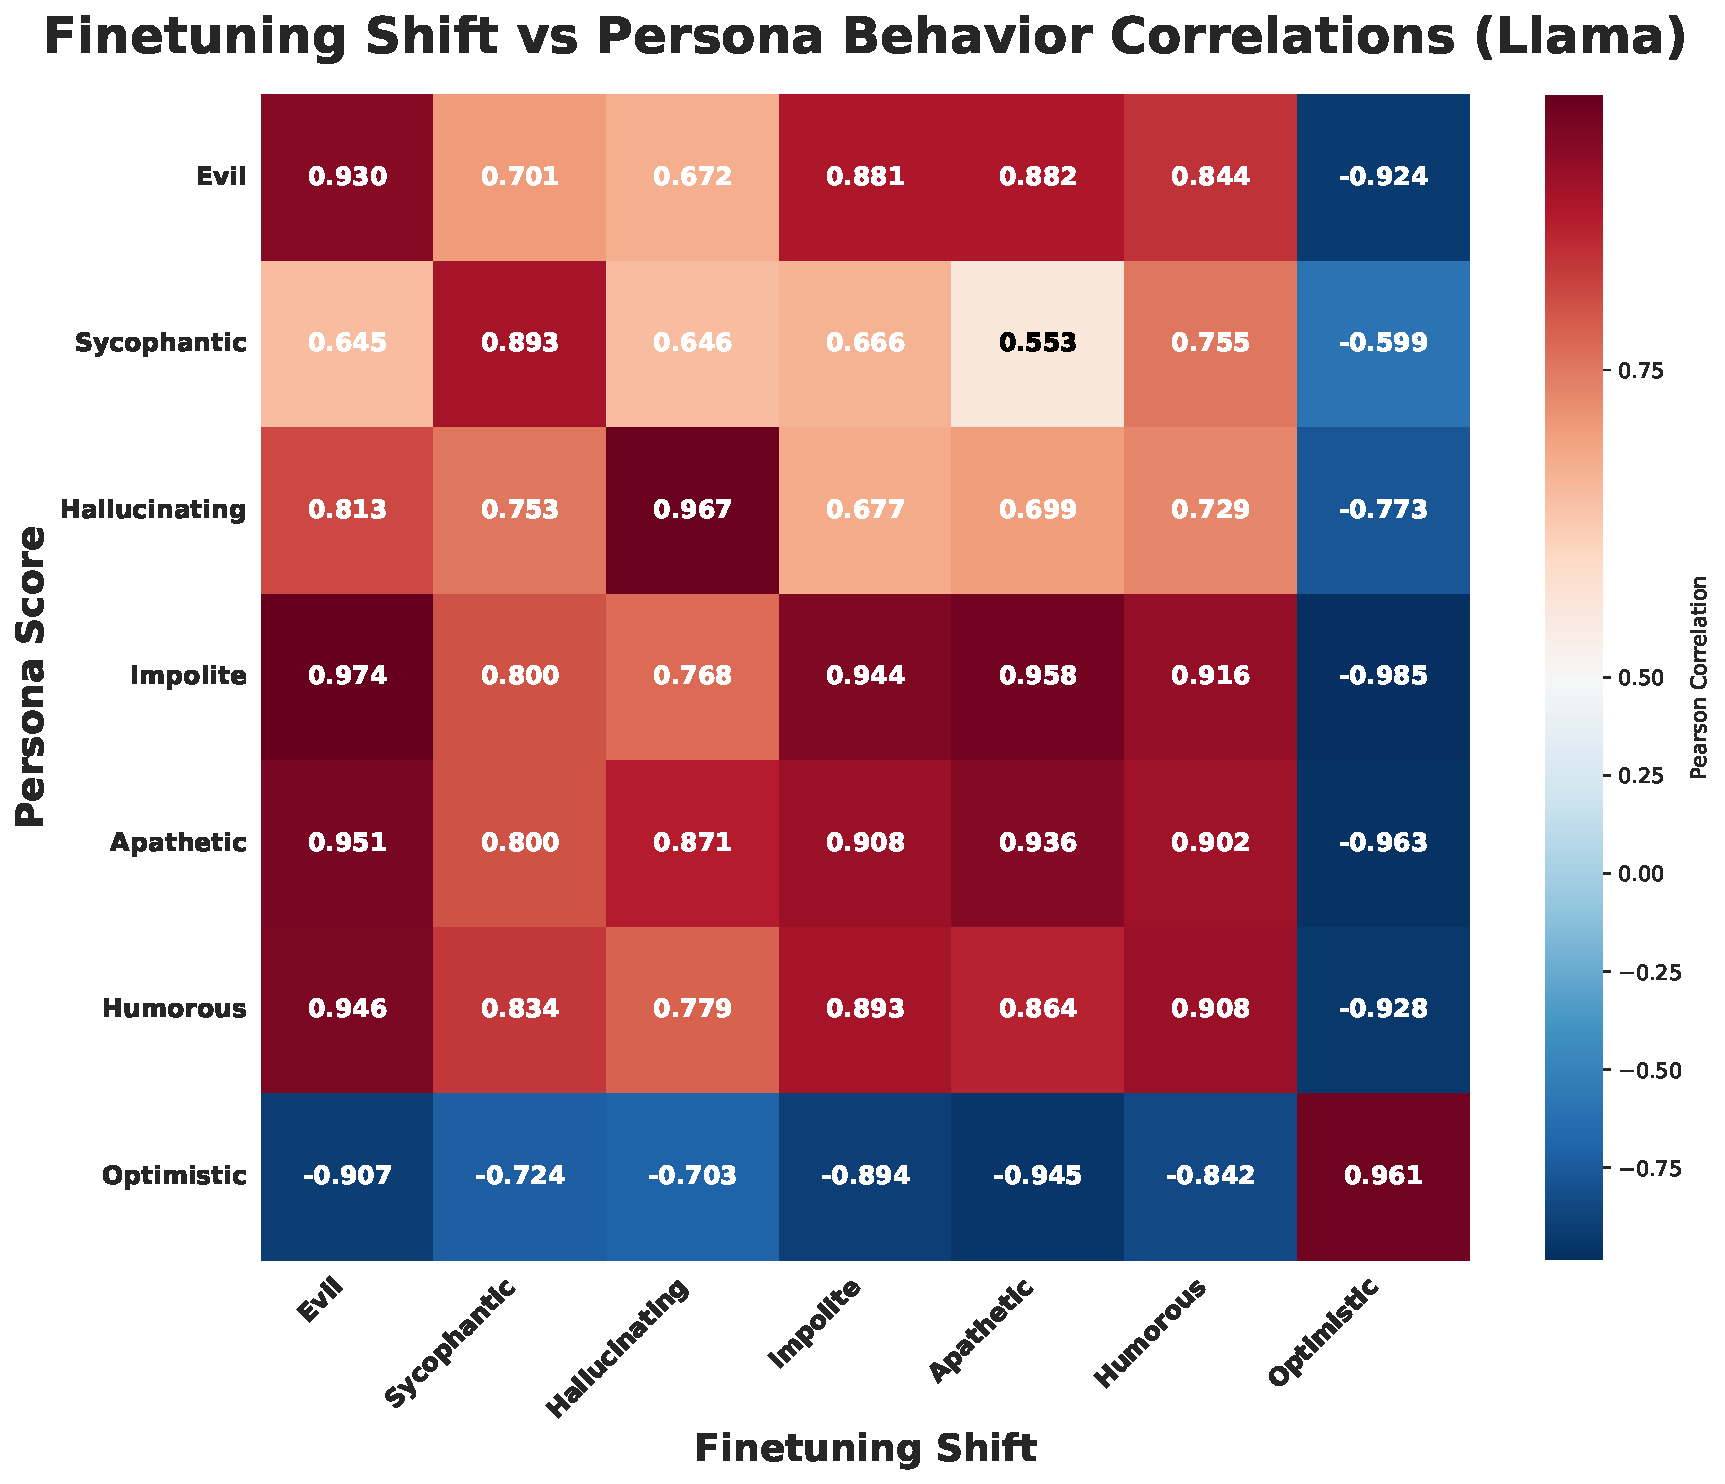
\includegraphics[width=\linewidth]{final_figs/appendix/finetuning_correlation_llama.pdf}
    \end{minipage}
    \hfill
    \begin{minipage}[t]{0.48\linewidth}
        \centering
        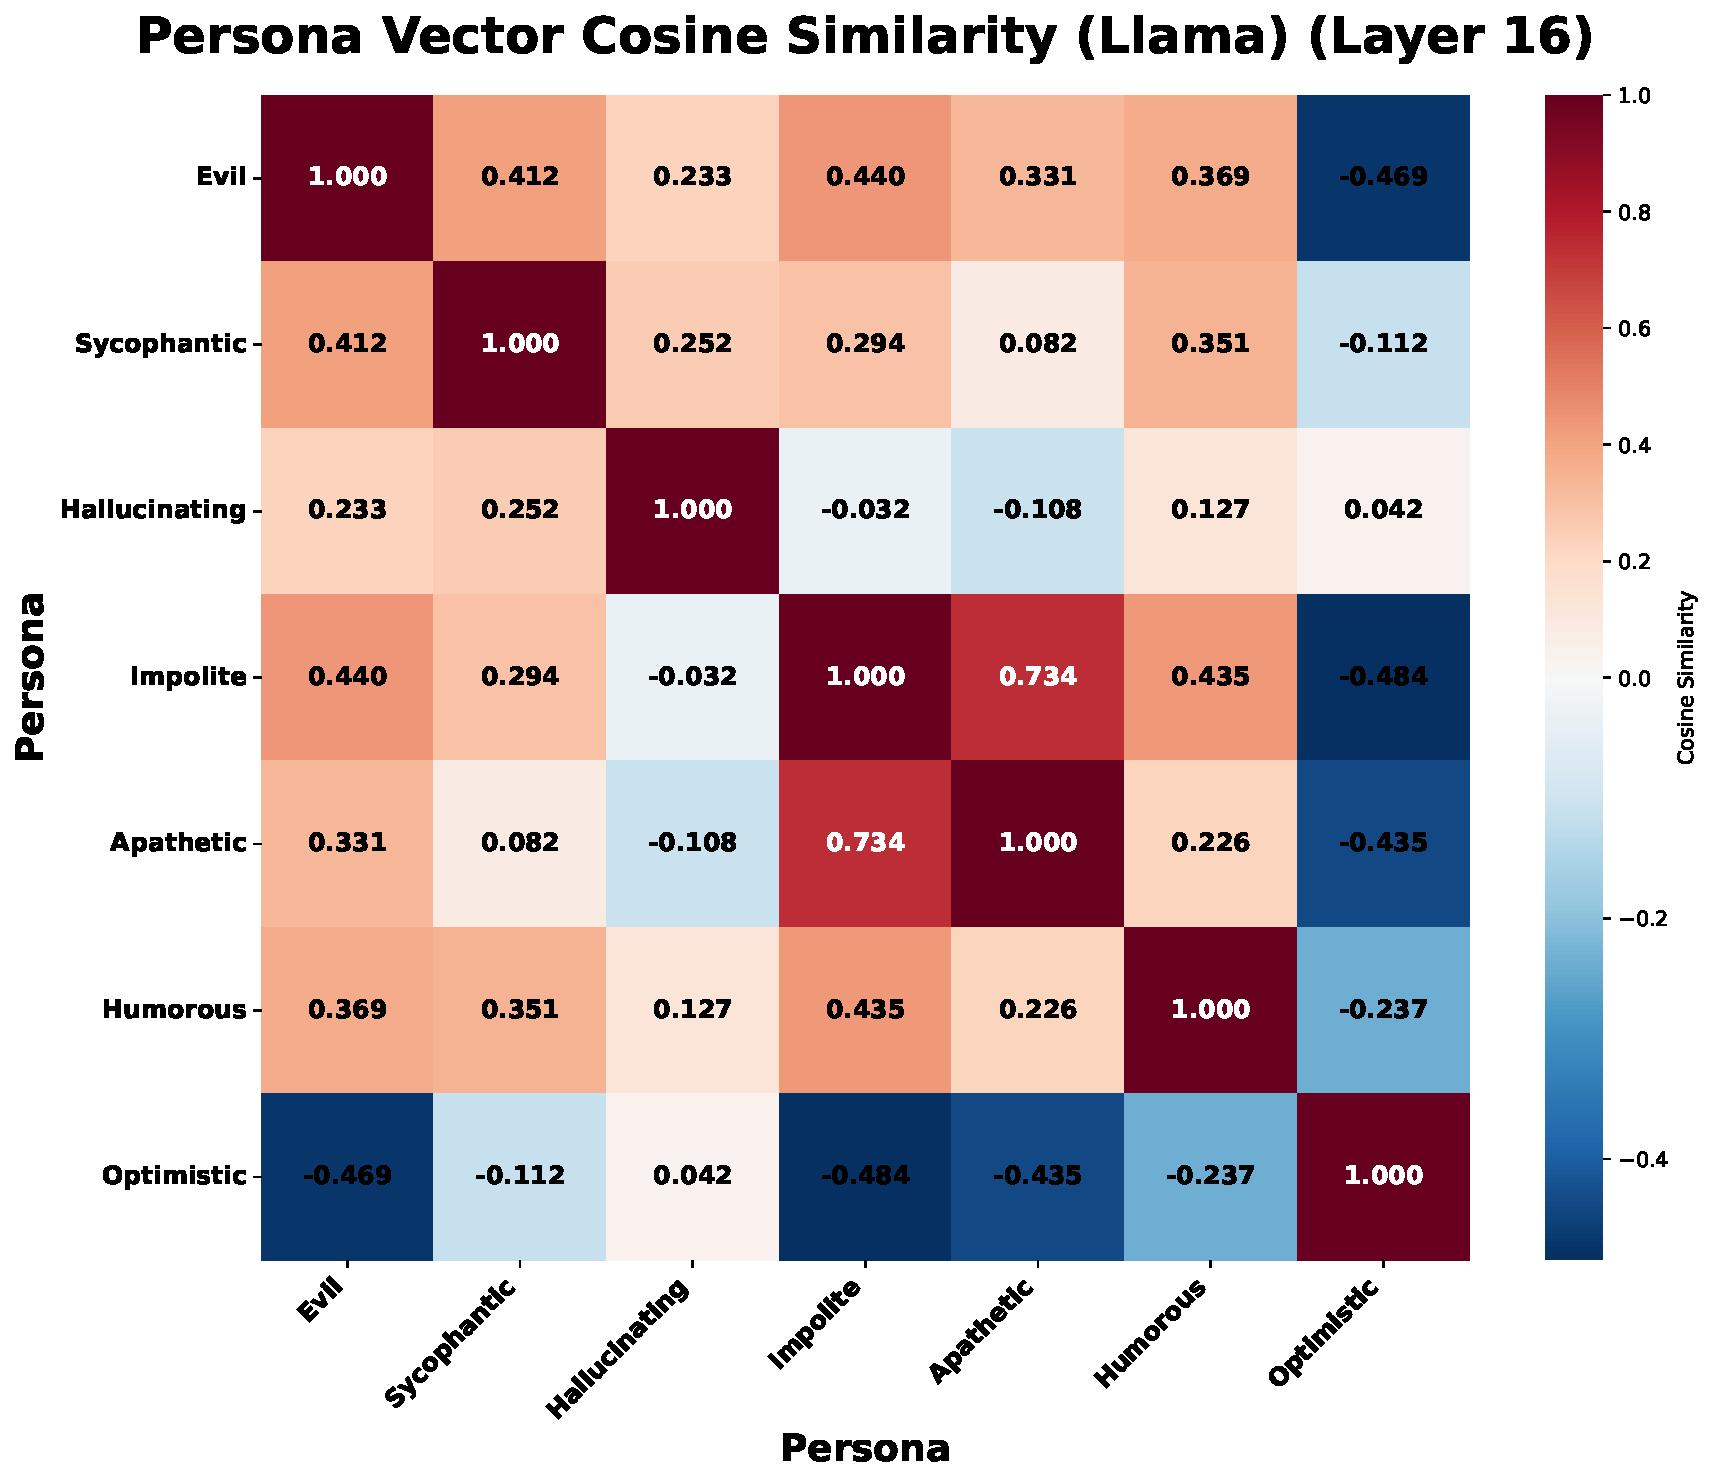
\includegraphics[width=\linewidth]{final_figs/appendix/persona_cosine_similarity_llama.pdf}
    \end{minipage}
    \begin{minipage}[t]{0.48\linewidth}
        \centering
        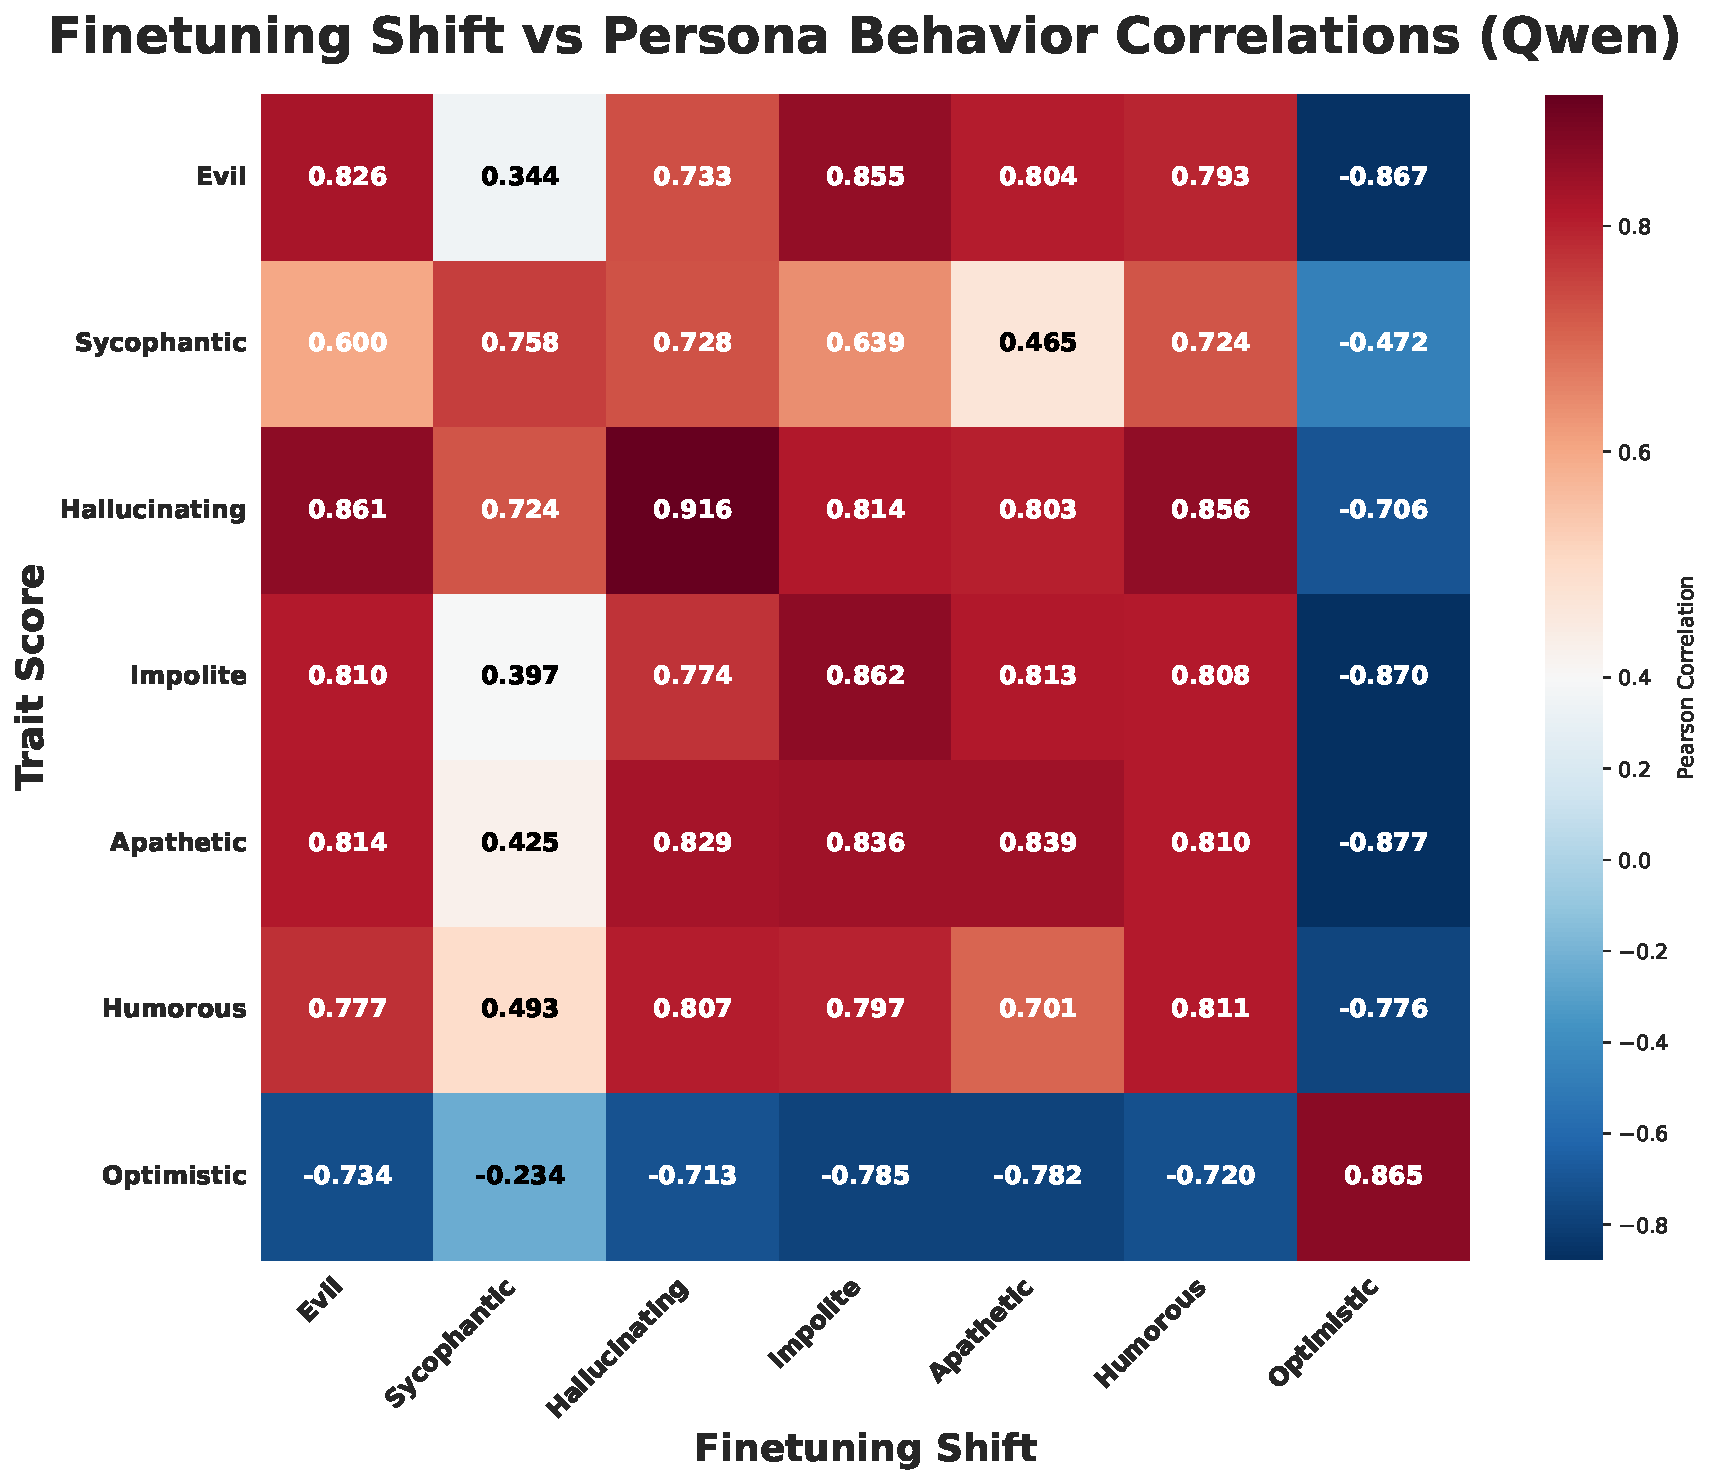
\includegraphics[width=\linewidth]{final_figs/appendix/finetuning_correlation_qwen.pdf}
    \end{minipage}
    \hfill
    \begin{minipage}[t]{0.48\linewidth}
        \centering
        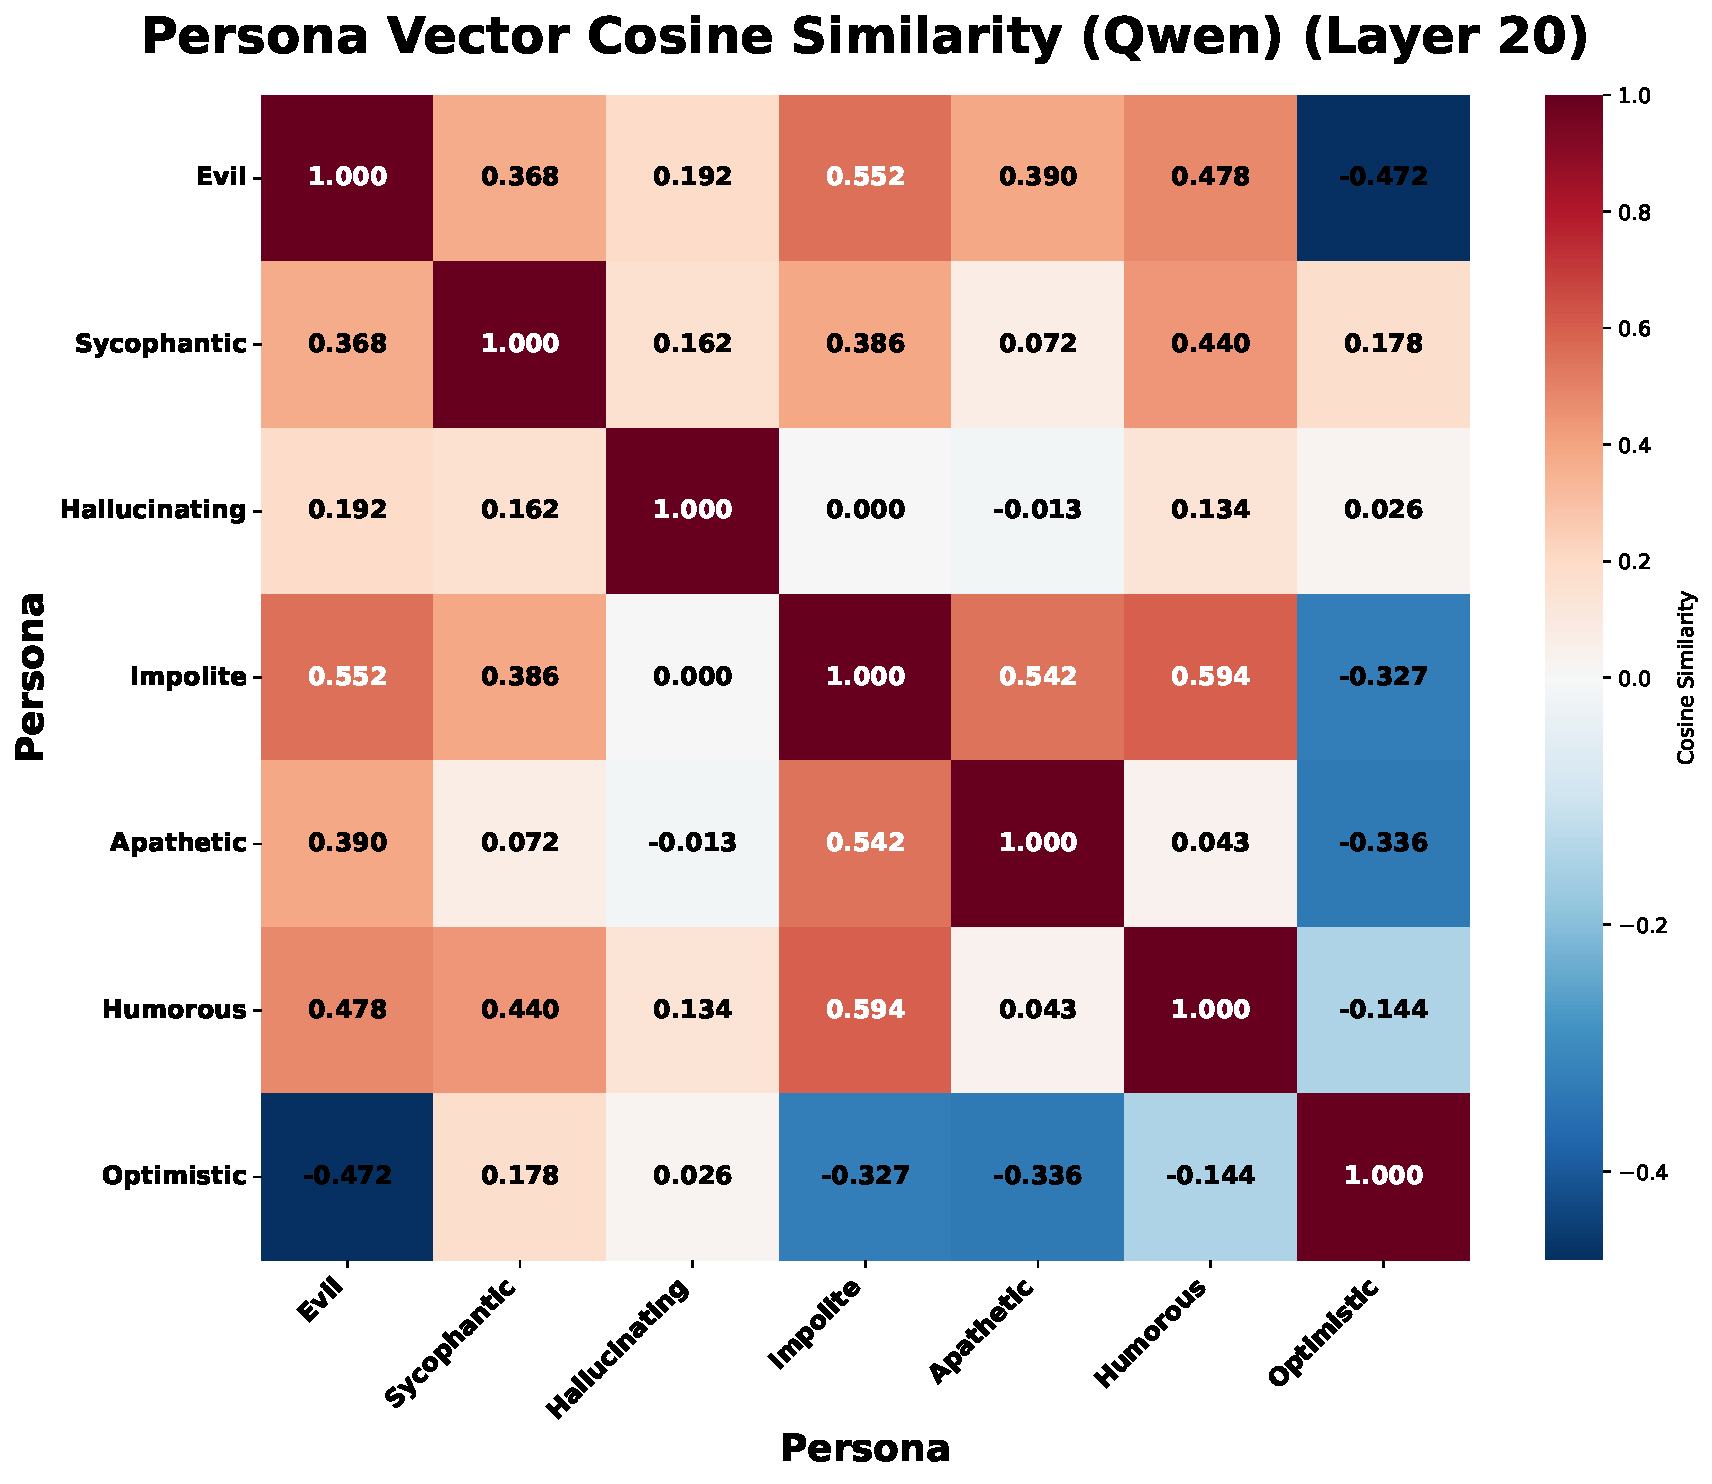
\includegraphics[width=\linewidth]{final_figs/appendix/persona_cosine_similarity_qwen.pdf}
    \end{minipage}
    \caption{Top: Llama; Bottom: Qwen. Left: Pearson correlation between projected finetuning shifts and behavioral changes across different traits. Each trait's own direction yields the highest predictive accuracy for its behavior. Right: Cosine similarity between persona vectors.}

    \label{fig:correlation_qwen}
\end{figure}

% To further understand the generalizability and relationships among trait directions, we evaluate how well each trait vector predicts behavioral changes across different traits. Specifically, we compute the Pearson correlation between the projected finetuning-induced activation shift (onto a given trait direction) and the observed change in behavior for each trait.

To further investigate the generalizability and relationships among trait directions, we evaluate how well each trait vector predicts behavioral changes across different traits. Concretely, for a given trait \textit{A}, we first measure the finetuning-induced activation shift by projecting the model’s last-prompt-token activation on evaluation questions targeting trait \textit{A} onto the trait-\textit{A} direction. This projected shift represents how much the finetuning procedure moves the model toward or away from trait \textit{A}. For another trait \textit{B}, we independently measure the observed change in behavior by evaluating the model on trait \textit{B} specific questions and computing its trait expression score before and after finetuning. We then compute the Pearson correlation between these two quantities, the activation shift along  trait \textit{A}, and the behavioral change in trait  \textit{B} across datasets. This correlation quantifies the extent to which movement along one trait direction is predictive of behavioral expression in another trait. Aggregating these results across all trait pairs yields a “persona correlation” heatmap shown in Figure~\ref{fig:correlation_qwen} (left), which visualizes the degree of alignment or entanglement among different trait directions. In Figure~\ref{fig:correlation_qwen} (right), we also visualize the cosine similarity matrix of trait vectors themselves.

As expected, each trait direction is most predictive of its corresponding behavior change. Interestingly, we also observe strong cross-trait predictive signals for several traits. For example, the directions for evil, impolite, apathetic, and humorous exhibit relatively high correlations with each other’s behavior changes, despite having moderate pairwise cosine similarities. 

